\documentclass[lettersize,journal]{IEEEtran}
\usepackage{amsmath,amsfonts}
\usepackage{algorithmic}
\usepackage{algorithm}
\usepackage{array}
\usepackage[caption=false,font=normalsize,labelfont=sf,textfont=sf]{subfig}
\usepackage{textcomp}
%\usepackage{stfloats}  % Package not available - commented out
\usepackage{url}
\usepackage{verbatim}
\usepackage{graphicx}
\usepackage{cite}
\hyphenation{op-tical net-works semi-conduc-tor IEEE-Xplore}
% updated with editorial comments 8/9/2021

\begin{document}

\title{3DGS: Un acercamiento al fotorrealismo}

\author{Alejandro Caicedo}

% The paper headers
\markboth{Pontificia Universidad Javeriana}%
{Shell \MakeLowercase{\textit{et al.}}: A Sample Article Using IEEEtran.cls for IEEE Journals}

\IEEEpubid{}
% Remember, if you use this you must call \IEEEpubidadjcol in the second
% column for its text to clear the IEEEpubid mark.

\maketitle

\begin{abstract}
Este artículo presenta una revisión de la técnica de esparcimiento gaussiano 3D (3DGS) como método de reconstrucción y renderización de escenas tridimensionales fotorrealistas. Se explora el funcionamiento de 3DGS y sus aplicaciones en plataformas comerciales como Meta Horizon Hyperscape y BRINK Traveler. Además, se identifican las principales limitaciones incluyendo requisitos de escenas estáticas, desafíos en la extracción de geometría, y obstáculos para su integración en aplicaciones interactivas y dinámicas.
\end{abstract}

\begin{IEEEkeywords}
Gaussian Splatting, Esparcimiento Gaussiano, Fotogrametría, Computación Gráfica, Realidad Virtual, 3DGS.
\end{IEEEkeywords}

\section{Introducción}
\IEEEPARstart{L}{a} reconstrucción de objetos reales para ser representados en aplicaciones gráficas ha sido uno de los problemas más estudiados en el campo de la computación gráfica. En los últimos años, la fotogrametría ha emergido como una técnica efectiva para capturar la geometría y apariencia de objetos del mundo real. Una de las técnicas más prometedoras en este ámbito es el esparcimiento gaussiano (Gaussian Splatting), específicamente la implementación 3DGS \cite{Kerbl2023}, que ha demostrado resultados sobresalientes en la reconstrucción de escenas y objetos 3D \cite{Gudon2024,Cascarano2025,Lian2024} en términos de tiempo de procesamiento, calidad fotorrealista y facilidad de captura.

La capacidad de 3DGS para lograr renderizado en tiempo real con calidad visual excepcional ha permitido que recientemente se publiquen múltiples implementaciones en aplicaciones para consumidores finales que pueden desplegarse en dispositivos con rendimiento limitado como teléfonos inteligentes y visores de realidad virtual \textit{standalone}. Plataformas comerciales como Meta Horizon Hyperscape \cite{MetaHorizon} y BRINK Traveler \cite{BrinkXR} ejemplifican esta democratización de la tecnología.

Este artículo presenta una revisión del funcionamiento de 3DGS, sus aplicaciones actuales en plataformas comerciales, y las limitaciones que enfrenta la tecnología en su estado actual, incluyendo requisitos de escenas estáticas, desafíos en la extracción de geometría, y obstáculos para su integración en aplicaciones interactivas y dinámicas. El objetivo es proporcionar una perspectiva integral sobre el estado actual de esta tecnología emergente y sus direcciones futuras de desarrollo. 

\section{Fotogrametría y Gaussian Splatting}
La fotogrametría es una metodología que utiliza un conjunto de imágenes 2D capturadas desde diferentes ángulos para reconstruir la geometría tridimensional de un objeto o escena \cite{Matias2025}. Este proceso implica la identificación de puntos en común entre las imágenes, la estimación de la posición y orientación de la cámara, y la generación de una nube de puntos 3D que representa la superficie del objeto \cite{Luhmann2019}. La fotogrametría es ampliamente utilizada en diversas aplicaciones, incluyendo arqueología, topografía, arquitectura y efectos visuales en cine y videojuegos\cite{MetaHorizon, Scaniverse, BrinkXR}. El objetivo de esta técnica es capturar la mayor cantidad de detalles posibles del objeto o escena, permitiendo una representación precisa y realista en entornos virtuales \cite{Luhmann2019} sin una necesidad explícita de equipos especializados. Por esta razón, la fotogrametría se ha convertido en una herramienta popular para la creación de contenido 3D en diversos contextos, y se han desarrollado múltiples técnicas y algoritmos para mejorar la precisión y eficiencia del proceso de reconstrucción \cite{Matias2025}.

Una de estas técnicas es el esparcimiento gaussiano, que es un método de representación de escenas 3D que utiliza funciones gaussianas para modelar la densidad y color de los puntos en el espacio tridimensional \cite{Kerbl2023}. Estas funciones gaussianas, o ``splats", son esferas tridimensionales que tienen una distribución de densidad gaussiana y pueden superponerse para formar una representación continua de la escena \cite{Matias2025}.  Una de las ventajas de este método es su capacidad para representar detalles finos y texturas complejas de manera eficiente, gracias a que utiliza un acercamiento de renderización rápido, diferenciable y consciente de la vista, lo que permite filtrado anisotrópico. También usa \textit{Tile-Based Efficiency}, lo que le permite aprovecharse de algoritmos ya optimizados en los procesadores gráficos\cite{Kerbl2023}.

Además, el esparcimiento gaussiano es robusto frente a ruido y oclusiones en los datos de entrada, lo que lo hace adecuado para aplicaciones en entornos del mundo real donde las condiciones de captura pueden ser desafiantes \cite{Gudon2024}. Esto gracias a su capacidad para suavizar y fusionar información de múltiples vistas, lo que resulta en una representación más coherente y precisa de la escena \cite{Cascarano2025}. En resumen, el esparcimiento gaussiano es una técnica prometedora para la representación y renderización de escenas 3D, que ofrece ventajas significativas en términos de calidad visual y eficiencia computacional \cite{Kerbl2023}.
\section{Funcionamiento de 3DGS}

La intención de este artículo no es ahondar en gran detalle en el funcionamiento algorítmico y matemático de 3DGS. Sin embargo, es relevante realizar una explicación a un nivel más alto del flujo de procesamiento de las imágenes y cómo se llega de estas a una escena u objeto 3D. Si el lector quiere estudiar el tema con más profundidad se recomiendan \cite{Kerbl2023,Matias2025}. Como ya se ha visto, 3DGS es una técnica de representación y renderización de escenas 3D que utiliza funciones gaussianas para modelar la densidad y color de los puntos en el espacio tridimensional \cite{Kerbl2023}. El proceso consta de varias etapas.

\begin{figure}[!t]
\centering
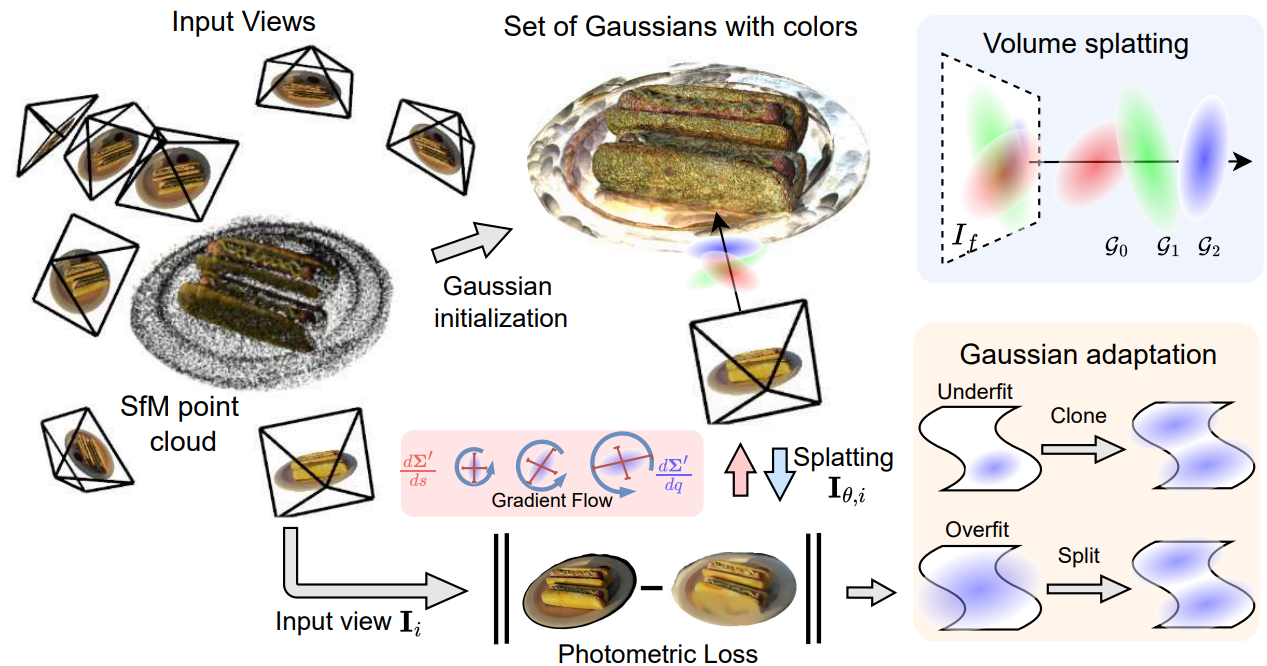
\includegraphics[width=3.4in]{fig1}
\caption{Flujo de procesamiento de 3DGS. Tomado de \cite{Kerbl2023}.}
\end{figure}

En primer lugar, se capturan múltiples imágenes 2D de la escena u objeto desde diferentes ángulos utilizando cámaras convencionales \cite{Matias2025}. Estas imágenes se utilizan como datos de entrada para el proceso de reconstrucción. A continuación, se realiza una calibración con respecto a las cámaras utilizadas para capturar las imágenes, lo que implica estimar la posición y orientación de cada cámara en el espacio tridimensional. Esta información es crucial para alinear correctamente las imágenes y garantizar una reconstrucción precisa de la escena.

Una vez completada la calibración de cámaras, se genera una nube de puntos dispersa mediante técnicas de fotogrametría tradicional, como Structure from Motion (SfM) \cite{Kerbl2023}. Esta nube de puntos inicial sirve como punto de partida para la optimización de las gaussianas 3D. Cada punto de la nube se convierte en una gaussiana 3D con propiedades como posición, covarianza (que define la forma y orientación), opacidad y coeficientes de armónicos esféricos que codifican el color dependiente de la vista \cite{Matias2025}.

El núcleo del proceso de 3DGS radica en la optimización iterativa de estas gaussianas para que coincidan con las imágenes capturadas \cite{Kerbl2023}. Durante esta fase, se proyectan las gaussianas en cada vista de cámara y se comparan los colores renderizados con los colores reales de las imágenes. La diferencia entre ambos se minimiza mediante técnicas de optimización basadas en gradientes, ajustando progresivamente las propiedades de cada gaussiana para mejorar la fidelidad visual de la reconstrucción.

Un aspecto fundamental de 3DGS es el control adaptativo de densidad, que permite añadir, eliminar o dividir gaussianas según sea necesario durante la optimización \cite{Kerbl2023}. Las regiones con detalles complejos requieren más gaussianas, mientras que las áreas uniformes pueden representarse con menos. Este mecanismo de control asegura que los recursos computacionales se utilicen eficientemente, concentrando la representación donde más se necesita.

El renderizado en 3DGS se realiza mediante un algoritmo de rasterización diferenciable que ordena las gaussianas de adelante hacia atrás con respecto a cada vista de cámara \cite{Matias2025}. Este proceso utiliza técnicas de \textit{tile-based rendering}, dividiendo la imagen en bloques pequeños y procesando solo las gaussianas que afectan a cada bloque. Esta estrategia permite aprovechar las capacidades de paralelización de las GPUs modernas, logrando tasas de renderización en tiempo real incluso para escenas complejas \cite{Kerbl2023}.

Finalmente, el resultado es una representación 3D completamente con un alto grado de optimización que puede ser renderizada desde cualquier punto de vista en tiempo real, manteniendo alta calidad visual y permitiendo aplicaciones interactivas \cite{Wu2024}.

\section{Aplicaciones actuales}

La técnica de esparcimiento gaussiano implementada en 3DGS ha encontrado aplicaciones en diversos campos, especialmente en aquellos que requieren la captura y representación precisa de objetos y escenas del mundo real. En esta sección se explorarán algunas de las aplicaciones actuales más relevantes a criterio del autor.
\subsection{Meta Horizon Hyperscape}

Meta, la empresa con uno de los mercados más grandes en el ámbito de la realidad virtual, ha integrado la tecnología de esparcimiento gaussiano en su plataforma Meta Horizon Hyperscape \cite{MetaHorizon}. Esta plataforma permite a los usuarios capturar y explorar entornos 3D detallados utilizando dispositivos de realidad virtual \textit{standalone}, como el Meta Quest 3 y 3S. La integración de 3DGS en Meta Horizon Hyperscape ha permitido a los usuarios crear representaciones realistas de sus entornos físicos, con un muy bajo nivel de dificultad técnica. La aplicación guía a los usuarios a través de un proceso sencillo de captura de imágenes en tres fases que utiliza las cámaras del dispositivo. Una vez capturadas las imágenes, la plataforma las sube a un servidor de Meta, donde se procesa la información utilizando 3DGS para generar una representación 3D optimizada. Los usuarios pueden luego explorar estos entornos en realidad virtual.

\begin{figure}[H]
\centering
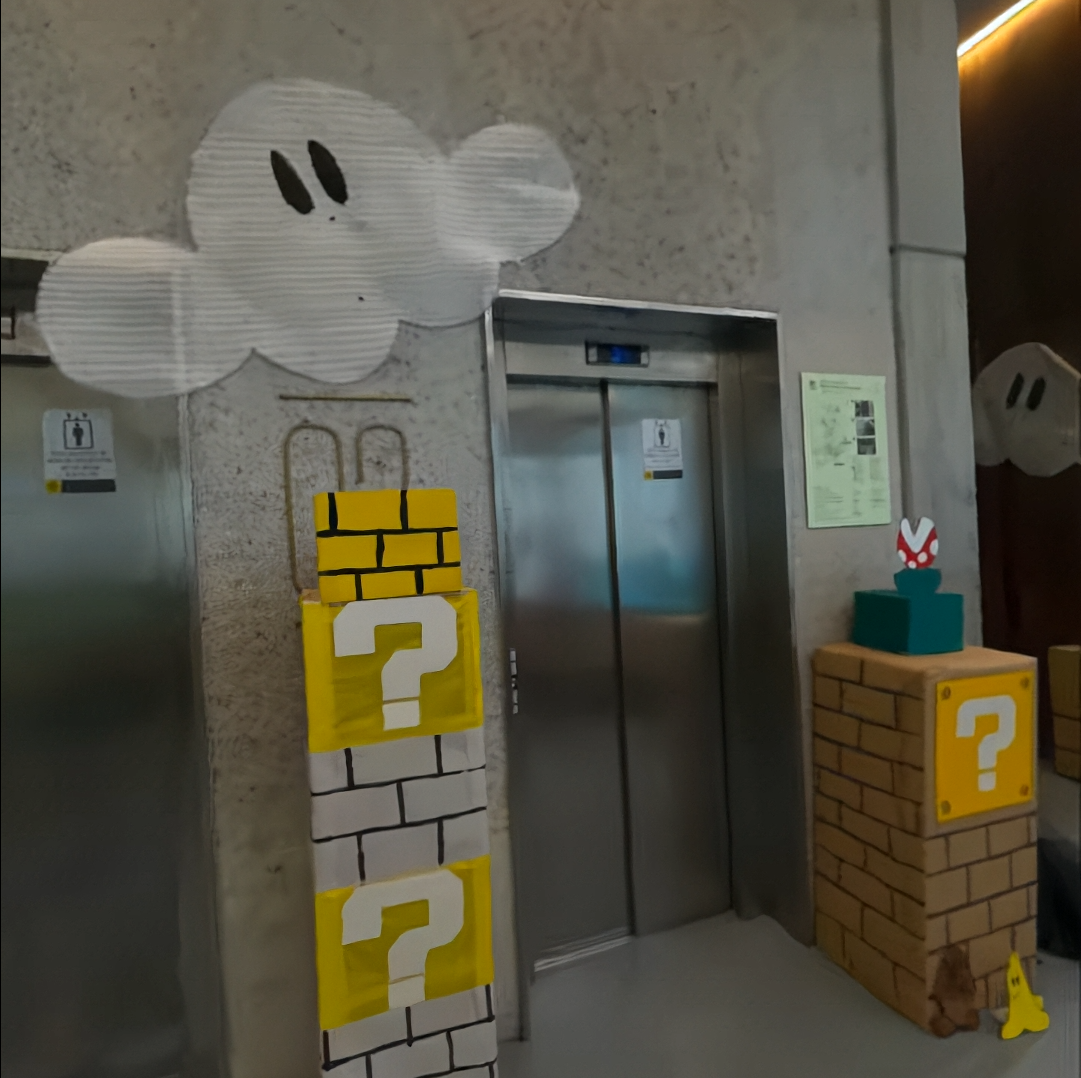
\includegraphics[width=3in]{fig2}
\caption{Captura de pantalla de Meta Horizon Hyperscape. En un dispositivo Meta Quest 3.}
\label{fig2}
\end{figure}

\begin{figure}[!t]
\centering
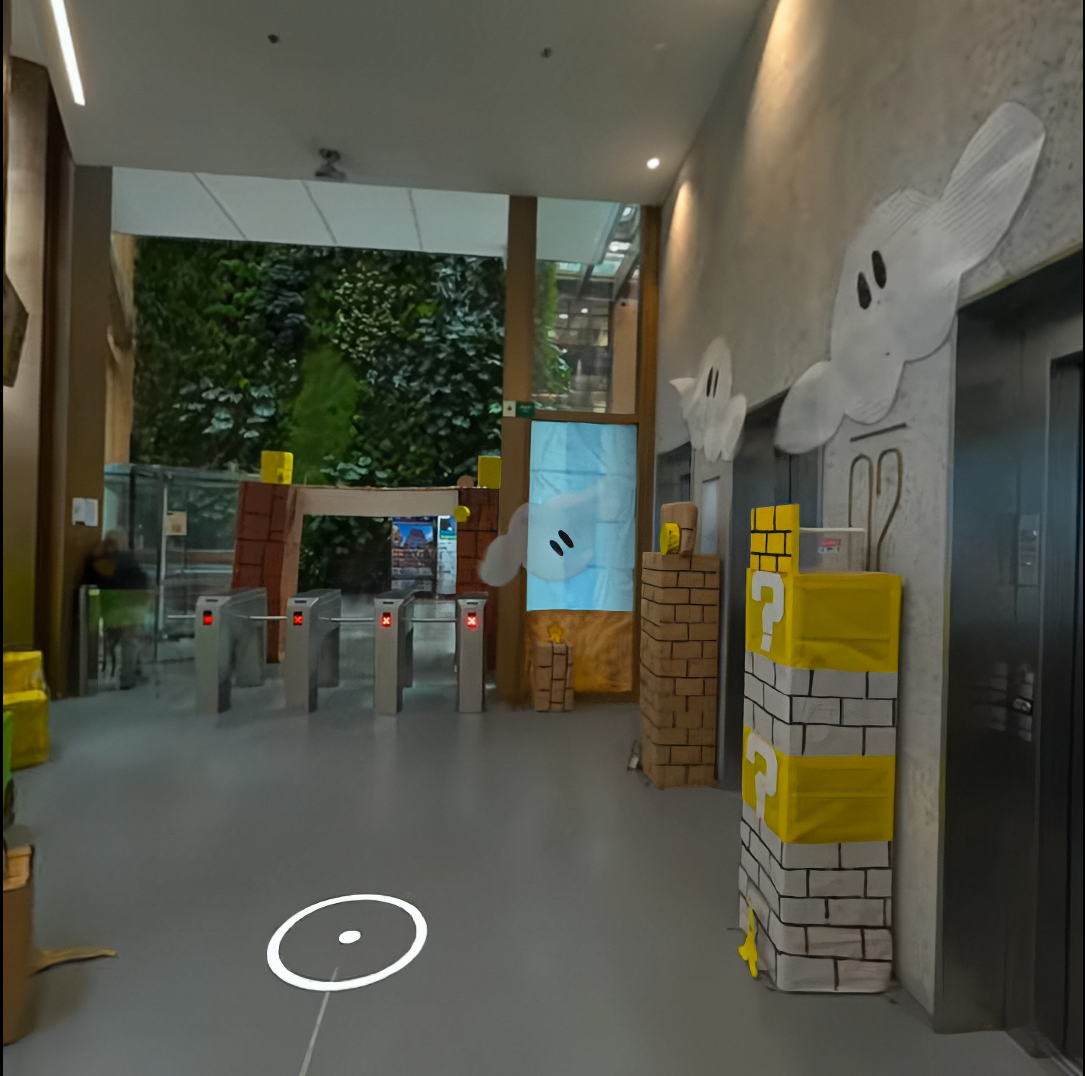
\includegraphics[width=3in]{fig3}
\caption{Captura de pantalla de Meta Horizon Hyperscape. En un dispositivo Meta Quest 3.}
\label{fig3}
\end{figure}

\begin{figure}[!t]
\centering
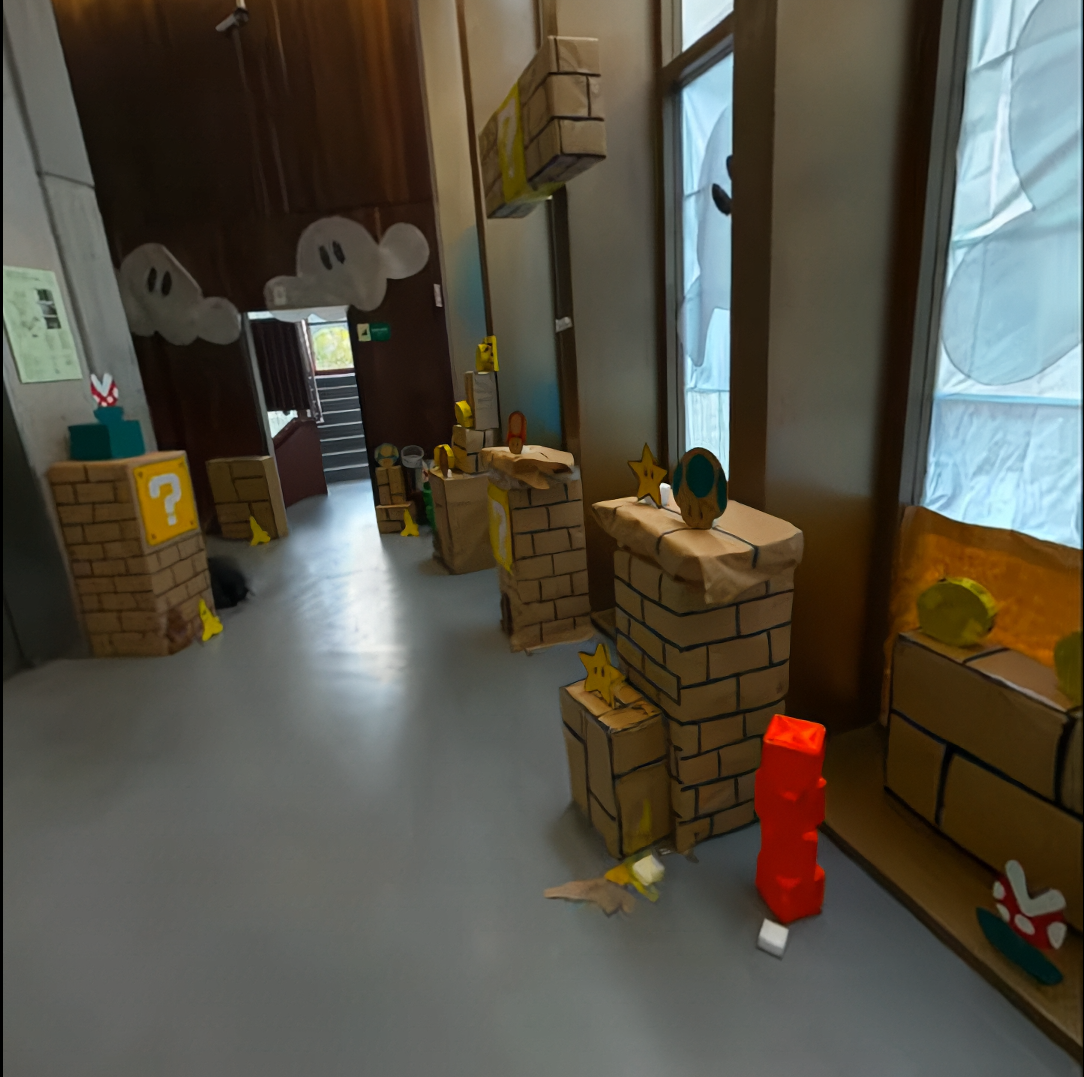
\includegraphics[width=3in]{fig4}
\caption{Captura de pantalla de Meta Horizon Hyperscape. En un dispositivo Meta Quest 3.}
\label{fig4}
\end{figure}

Las figuras \ref{fig2}, \ref{fig3} y \ref{fig4} muestran capturas de pantalla tomadas de una escena generada con Meta Horizon Hyperscape en un dispositivo Meta Quest 3. Estas imágenes fueron tomadas el día de Halloween de 2025 en el edificio de laboratorios de ingeniería de la Pontificia Universidad Javeriana. Dadas las limitaciones del formato, el artículo está limitado a imágenes estáticas. Sin embargo, el video a partir del cual se tomaron estas capturas puede encontrarse en \cite{HalloweenJaveriano2025}.

Se puede observar en las imágenes una representación detallada del entorno, con texturas y colores que reflejan con precisión casi fotorrealista la escena original. Además, hay una presencia baja de artefactos visuales, y los más visibles (Más aparentes en la figura \ref{fig4}) son causados por el movimiento de los objetos durante la captura de las imágenes, lo cual contamina los datos de entrenamiento. Esto es una de las limitaciones actuales de la técnica, ya que 3DGS asume que la escena es estática durante la captura. 

\subsection{BRINK Traveler}

BRINK Traveler \cite{BrinkXR} es una aplicación de viajes virtuales que utiliza captura volumétrica 3D para recrear lugares del mundo real con un nivel fotorrealista de detalle. La plataforma aprovecha tecnologías de reconstrucción 3D avanzadas, incluyendo esparcimiento gaussiano, para crear experiencias inmersivas que transportan a los usuarios a locaciones icónicas desde la comodidad de su hogar.

BRINK Traveler está disponible tanto para dispositivos de realidad virtual, incluyendo Meta Quest y headsets compatibles con SteamVR, como para dispositivos móviles a través de realidad aumentada en teléfonos y tabletas iOS y Android. Esta versatilidad hace que las experiencias sean accesibles a una audiencia amplia sin necesidad de hardware especializado costoso.

La aplicación ofrece experiencias completamente tridimensionales con seis grados de libertad (6DoF), permitiendo a los usuarios moverse a través de las locaciones capturadas como lo harían en persona. Una característica distintiva de BRINK Traveler es su enfoque social, que permite a usuarios de diferentes partes del mundo compartir estas experiencias simultáneamente, creando oportunidades para explorar juntos lugares remotos. Además, cada locación ofrece elementos interactivos que van más allá de la simple observación, proporcionando información educativa y permitiendo a los usuarios interactuar con el entorno virtual.

\subsection{Scaniverse}

Scaniverse \cite{Scaniverse} es una aplicación móvil y de XR que permite a los usuarios capturar, editar y compartir modelos 3D de alta calidad utilizando la cámara de su dispositivo. La aplicación utiliza técnicas avanzadas de fotogrametría y esparcimiento gaussiano para generar representaciones tridimensionales detalladas de objetos y escenas del mundo real. 

Una de las características más destacadas de Scaniverse es su capacidad para realizar capturas rápidas, precisas y procesadas en el dispositivo. Los usuarios pueden simplemente apuntar la cámara de su dispositivo hacia el objeto o escena que desean capturar y mover el dispositivo alrededor para obtener múltiples vistas. La aplicación procesa estas imágenes utilizando algoritmos de esparcimiento gaussiano para crear un modelo 3D optimizado que puede ser visualizado y manipulado directamente en el dispositivo.

Scaniverse también ofrece herramientas de edición integradas que permiten a los usuarios ajustar la geometría, texturas y otros aspectos del modelo 3D antes de compartirlo en plataformas sociales o exportarlo para su uso en otras aplicaciones. Dado que la aplicación soporta exportar en formatos estándar como OBJ y GLTF, los modelos creados pueden ser fácilmente integrados en flujos de trabajo de diseño 3D, realidad aumentada y realidad virtual.


\section{Limitaciones}

A pesar de los avances significativos que ha logrado la técnica de esparcimiento gaussiano en la síntesis de vistas novedosas y la representación 3D de escenas, existen varias limitaciones importantes que deben ser consideradas tanto en su implementación como en sus aplicaciones prácticas.

\subsection{Requisitos de escenas estáticas}

Una de las limitaciones más fundamentales de 3DGS es su asunción de que la escena capturada permanece completamente estática durante el proceso de adquisición de imágenes \cite{Kerbl2023}. Esta restricción implica que cualquier movimiento de objetos, personas o elementos dentro de la escena durante la captura puede generar artefactos visuales significativos en la reconstrucción final. El movimiento contamina el conjunto de datos de entrenamiento, resultando en inconsistencias geométricas y visuales que degradan la calidad de la representación \cite{Matias2025}. Esta limitación es particularmente problemática en entornos reales donde resulta difícil o imposible garantizar la ausencia total de movimiento, como en espacios públicos, exteriores con vegetación, o escenarios con presencia humana.

Aunque trabajos recientes como 4D Gaussian Splatting \cite{Wu2024} han propuesto extensiones para manejar escenas dinámicas mediante la incorporación de una dimensión temporal, estas soluciones aumentan significativamente la complejidad computacional y los requisitos de almacenamiento. La representación de escenas dinámicas requiere codificar las deformaciones de los gaussianos a través del tiempo, lo que implica un proceso de optimización más complejo y costoso en términos de memoria y procesamiento.

\subsection{Desafíos en la extracción de geometría}

Otra limitación importante radica en la dificultad inherente para extraer mallas geométricas precisas a partir de la representación de gaussianos 3D \cite{Gudon2024}. Después del proceso de optimización, los millones de gaussianos que componen la escena tienden a estar desorganizados y no necesariamente alineados con las superficies reales de los objetos. Esta característica dificulta la obtención de modelos de malla tradicionales que son esenciales para muchas aplicaciones de gráficos por computador, incluyendo edición, esculpido, animación y reluminación.

Métodos como SuGaR \cite{Gudon2024} han abordado este problema introduciendo términos de regularización que incentivan la alineación de los gaussianos con las superficies de la escena, permitiendo posteriormente la extracción de mallas mediante técnicas como la reconstrucción de Poisson. Sin embargo, este proceso adicional requiere tiempo de procesamiento extra y puede introducir compromisos entre la fidelidad visual y la calidad geométrica de la malla resultante.

\subsection{Limitaciones en la captura y digitalización}

Los estudios comparativos entre diferentes métodos de reconstrucción 3D \cite{Cascarano2025, Doma2025} han revelado que, aunque 3DGS ofrece ventajas significativas en términos de calidad visual y eficiencia de renderizado, enfrenta desafíos específicos relacionados con el proceso de captura. La calidad de la reconstrucción depende críticamente de la cantidad y calidad de las imágenes de entrada, la cobertura adecuada de todos los ángulos de la escena, y las condiciones de iluminación durante la captura.

En comparación con métodos de escaneo estructurado como Artec Eva o tecnologías LiDAR, que proporcionan mediciones directas de profundidad, 3DGS depende exclusivamente de técnicas fotogramétricas que reconstruyen la geometría a partir de múltiples vistas \cite{Luhmann2019}. Esta dependencia implica que superficies con texturas uniformes, materiales reflectantes o transparentes, y áreas con iluminación insuficiente o inconsistente pueden resultar en reconstrucciones de baja calidad o incompletas.

\subsection{Requisitos computacionales y de almacenamiento}

Aunque 3DGS es considerablemente más eficiente que otros métodos para el renderizado en tiempo real, la representación mediante millones de gaussianos 3D implica requisitos sustanciales de memoria y almacenamiento \cite{Kerbl2023, Wu2024}. Cada gaussiano debe almacenar múltiples parámetros incluyendo posición, color, opacidad y covarianza anisotrópica, lo que puede resultar en modelos con tamaños de archivo considerables para escenas complejas o de gran escala.

Además, el proceso de optimización durante el entrenamiento requiere hardware con capacidades gráficas significativas, particularmente memoria GPU suficiente para manejar millones de primitivas simultáneamente. Esto puede limitar la accesibilidad de la tecnología para usuarios sin acceso a hardware especializado de alto rendimiento.

\subsection{Desafíos en aplicaciones interactivas y dinámicas}

En el contexto de aplicaciones interactivas como videojuegos, simuladores y experiencias de realidad virtual o aumentada, existen limitaciones relacionadas con la integración de contenido basado en gaussianos con elementos dinámicos del entorno. La naturaleza fundamentalmente estática de las representaciones 3DGS dificulta la implementación de modificaciones en tiempo real, la interacción directa con objetos específicos dentro de la escena reconstruida, o la simulación de comportamientos físicos dinámicos.

Para aplicaciones que requieren manipulación de objetos, detección de colisiones y modificación procedimental de escenas, la representación mediante gaussianos presenta desafíos particulares. La dificultad para extraer geometría explícita \cite{Gudon2024} complica la implementación de mecánicas tradicionales que dependen de mallas poligonales para física y navegación. Aunque extensiones como 4D Gaussian Splatting \cite{Wu2024} permiten representar movimiento y deformaciones, estas técnicas aumentan significativamente la complejidad computacional.

El renderizado de escenas complejas con millones de gaussianos en dispositivos con recursos limitados, como headsets de realidad virtual \textit{standalone} \cite{MetaHorizon, Lian2024}, presenta desafíos de rendimiento adicionales debido a las limitaciones de procesamiento y memoria. Esto requiere compromisos entre calidad visual y rendimiento para mantener tasas de refresco adecuadas. Adicionalmente, la integración de elementos sintéticos generados por computadora con escenas capturadas mediante 3DGS presenta desafíos de coherencia visual e iluminación que aún están en desarrollo activo.

\section{Conclusiones}

La técnica de esparcimiento gaussiano 3D representa un avance significativo en la reconstrucción y renderización de escenas fotorrealistas, superando a técnicas previas como NeRF en velocidad de entrenamiento y capacidad de renderizado en tiempo real \cite{Kerbl2023}. Su adopción en aplicaciones comerciales como Meta Horizon Hyperscape \cite{MetaHorizon} y BRINK Traveler \cite{BrinkXR} demuestra la viabilidad de la tecnología en dispositivos de consumo masivo.

Sin embargo, 3DGS enfrenta limitaciones importantes: la dependencia de escenas estáticas \cite{Kerbl2023, Matias2025}, dificultades en la extracción de geometría explícita \cite{Gudon2024}, requisitos computacionales sustanciales, y obstáculos para la integración en aplicaciones interactivas. A pesar de estos desafíos, el desarrollo continuo de extensiones como 4D Gaussian Splatting \cite{Wu2024} y métodos mejorados de extracción de mallas \cite{Gudon2024} sugieren perspectivas prometedoras.

En conclusión, 3DGS ha establecido un nuevo estándar en la representación de escenas tridimensionales, ofreciendo un balance único entre calidad visual, eficiencia computacional y accesibilidad. A medida que la tecnología madura, es probable que desempeñe un papel cada vez más importante en aplicaciones que van desde la preservación cultural y educación hasta el entretenimiento, contribuyendo significativamente a la evolución de las experiencias inmersivas.

\bibliographystyle{IEEEtran}
\bibliography{ArticuloGaussianSplatting}

\end{document}


